\section{Generalità sul processore}
Il processore, di per se, è un componente atto ad eseguire dei codici operativi predefiniti all'interno della sua ISA.
Oltre al codice operativo, in un processore, vi è anche la sua \textbf{architettura}, che può essere di vario tipo. In generale un processore, a livello architetturale, è formata dai seguenti componenti:
\begin{itemize}
    \item \textbf{Unità di controllo}: Determina i passi elementari che deve fare un processore al fine di eseguire un istruzione;
    \item \textbf{Registro Program Counter}: Registro contenente il puntatore alla prossima istruzione;
    \item \textbf{Registro Istruction Register}: Registro contenente l'istruzione che sta venendo eseguita;
    \item \textbf{Registro Memory Address}: Registro di interfacciamento con la memoria, per gli indirizzi;
    \item \textbf{Registro Memory Buffer}: Registro di interfacciamento della memoria, per i dati;
    \item \textbf{Registri dato ad uso generico}: Registri dato e indirizzo presenti nell'architettura;
    \item \textbf{Unità Logico-Aritmetica (ALU)}: Unità che permette le esecuzioni, dati gli operandi, di operazioni logico-aritmetiche.
\end{itemize}

In particolare, per l'\textbf{Unità Logico Aritmetica}, vi è un'interazione anche con un altro registro all'interno della stessa architettura, ovvero il registro di \textbf{stato} o \textbf{Status Register (SR)}, tale interazione è legata alle caratteristiche principali che può avere un risultato di un operazione aritmetica (\ref{par:salto}).

\uppercase{è} possibile visualizzare una pseudoarchitettura del processore all'interno dell'immagine [\ref{img:processore}]

\begin{figure}
    \centering
    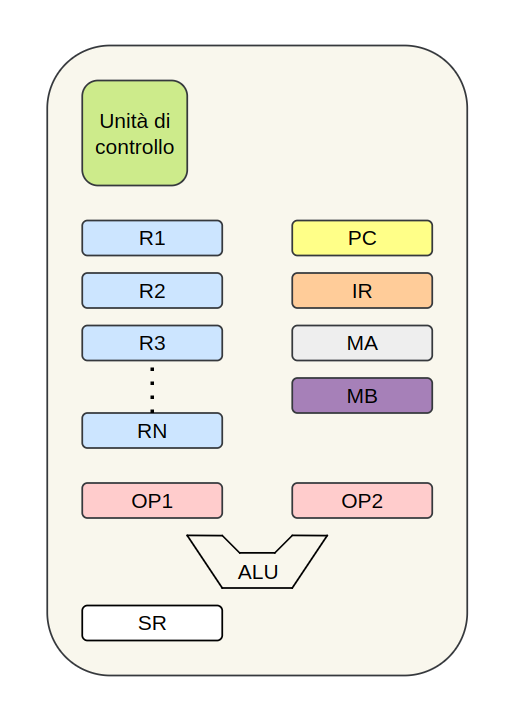
\includegraphics[width=.5\textwidth]{img/processore.png}
    \caption{Architettura di un processore generico}\label{img:processore}
\end{figure}

Oltre che la sua architettura interna, il processore è caratterizzato anche dal flusso di esecuzione di una specifica istruzione. Tale flusso può cambiare di architettura in architettura e sarà oggetto di approfondimento per i prossimi paragrafi.